% \iffalse meta-comment
% A class for preparing FP7 proposals for collaborative projects
%
% Copyright (c) 2011 Michael Kohlhase, all rights reserved
%
% This file is distributed under the terms of the LaTeX Project Public
% License from CTAN archives in directory  macros/latex/base/lppl.txt.
% Either version 1.0 or, at your option, any later version.
%
% The development version of this file can be found at
% https://github.com/KWARC/LaTeX-proposal
% \fi
% 
% \iffalse
%<cls|pdata|reporting>\NeedsTeXFormat{LaTeX2e}[1999/12/01]
%<cls>\ProvidesClass{euproposal}[2019/03/21 v1.5 EU Proposal]
%<pdata>\ProvidesPackage{eupdata}[2019/03/21 v1.5 EU Project Data]
%<reporting>\ProvidesPackage{eureporting}[2019/03/21 v1.5 EU Project Reporting]
%<*driver>
\documentclass[twoside]{ltxdoc}
\DoNotIndex{\def,\long,\edef,\xdef,\gdef,\let,\global}
\DoNotIndex{\begin,\AtEndDocument,\newcommand,\newcounter,\stepcounter}
\DoNotIndex{\immediate,\openout,\closeout,\message,\typeout}
\DoNotIndex{\section,\scshape,\arabic}
\EnableCrossrefs
%\CodelineIndex
%\OnlyDescription
\RecordChanges
\usepackage{textcomp,url,paralist,a4wide,xspace}
\usepackage[show]{ed}
\usepackage[maxbibnames=6,hyperref=auto,style=alphabetic,backend=bibtex]{biblatex}
\addbibresource{../lib/proposal.bib}
\usepackage[bookmarks=true,linkcolor=blue,
 citecolor=blue,urlcolor=blue,colorlinks=true,
 breaklinks=true, bookmarksopen=true]{hyperref}
\makeindex
\newcommand\subversion{\textsc{Subversion}\xspace}
\begin{document}
\DocInput{euproposal.dtx}
\end{document}
%</driver>
% \fi
% 
%\iffalse\CheckSum{639}\fi
% 
% \changes{v0.1}{2007/05/07}{used in the SciML proposal}
% \changes{v0.2}{2007/05/09}{First Version with Documentation}
% \changes{v0.3}{2007/06/04}{staff effort table finally works, released}
% \changes{v0.3a}{2008/01/18}{error corrections and more documentation}
% \changes{v1.3}{2011/05/18}{basing this on proposal.cls}
% \changes{v1.4}{2012/01/18}{various tweaks for the Jan 2012 proposal deadline}
% \changes{v1.4}{2015/01/14}{lots of tweaks}
% 
% \GetFileInfo{euproposal.cls}
% 
% \MakeShortVerb{\|}
% \title{Preparing FP7 EU Proposals and Reports in {\LaTeX} with \texttt{euproposal.cls}}
%    \author{Michael Kohlhase\\
%      Computer Science, Jacobs University Bremen\\
%      \url{http://kwarc.info/kohlhase}}
% \maketitle
%
% \begin{abstract}
%   The |euproposal| class supports many of the specific elements of a Framework 7
%   Proposal. It is optimized towards collaborative projects. The package comes with an
%   extensive example (a fake EU proposal) that shows all elements in action. 
% \end{abstract}
% 
% \tableofcontents\newpage
%
% \section{Introduction}\label{sec:intro}
%
%   Writing grant proposals is a collaborative effort that requires the integration of
%   contributions from many individuals. The use of an ASCII-based format like {\LaTeX}
%   allows to coordinate the process via a source code control system like
%   \subversion, allowing the proposal writing team to concentrate on the contents
%   rather than the mechanics of wrangling with text fragments and revisions. 
% 
%   The |euproposal| class extends the |proposal| class~\cite{Kohlhase:pplp:svn} and
%   supports many of the specific elements of Part B of a Framework 7 Proposal. The
%   package documentation is still preliminary, fragmented and incomplete and only dwells
%   on the particulars of DFG proposals, so we treat~\cite{Kohlhase:pplp:svn} as a
%   prerequisite. Please consult the example proposal |propB.tex|, which comes with the
%   package and shows the usage of the class in action. It is intended as a template for
%   your proposal, but please bear in mind that the EU guidelines may change from call to
%   call, if in doubt, please consult the FP7 guide for proposers.\ednote{say something
%   about the proposers guide.}
%
%   The |eureporting| class supports most of the specific elements of the project reports
%   to the EC. The example report |dfg/report.tex| is intended as a template for your
%   final report\ednote{say something about reporting}.
%
%   The |euproposal| and |eureporting| classes and the |eupdata| package are distributed
%   under the terms of the LaTeX Project Public License from CTAN archives in directory
%   macros/latex/base/lppl.txt.  Either version 1.0 or, at your option, any later
%   version. The CTAN archive always contains the latest stable version, the development
%   version can be found at \url{https://github.com/KWARC/LaTeX-proposal}. For bug reports
%   please use the sTeX TRAC at \url{https://github.com/KWARC/LaTeX-proposal/issues}.
%   
% \section{The User Interface}\label{sec:user-interface}
% 
% In this section we will describe the functionality offered by the |euproposal| class
% along the lines of the macros and environments the class provides. Much of the
% functionality can better be understood by studying the functional example |proposal.tex|
% (and its dependents) that comes with the |euproposal| package in conjunction with the
% proposer's EU proposer's guidelines (we have included it as |***| for convenience into
% the package distribution).\ednote{MK@MK do that and talk about reporting as well.}
% 
% \subsection{Package Options}\label{sec:user:options}
%
% As usual in {\LaTeX}, the package is loaded by
% |\documentclass[|\meta{options}|]{euproposal}|, where |[|\meta{options}|]| is optional
% and gives a comma separated list of options specified in~\cite{Kohlhase:pplp:svn}.  Some
% versions EU proposals want non-standard numbering schemes (e.g. starting with
% \textbf{B...} since we are writing Part B.), this can be reached by giving the |propB|
% option. Finally the |split| option cases the |euproposal| to write a file |SPLIT.at|
% that can be used in the |Makefile| to split the final proposal |final.pdf| into a files
% |final123.pdf| and |final45.pdf| for submission in the EU system (often this has to be
% separated so that the submission system can count pages.)
% 
% \subsection{Proposal Metadata and Title page}\label{sec:user:metadata}
% 
% The metadata of the proposal is specified in the \DescribeEnv{proposal}|proposal|
% environment, which also generates the title page and the first section of the proposal
% as well as the last pages of the proposal with the signatures, enclosures, and
% references. The |proposal| environment should contain all the mandatory parts of the
% proposal text. The |proposal| environment uses the following EU-specific keys to
% specify metadata.
% \begin{compactitem}
% \item \DescribeMacro{callname}|callname| specifies the call the proposal addresses. It is
%   usually a string of the form |ICT Call 1|, \DescribeMacro{callid}|callid| is the
%   corresponding identifier, usually a string of the form |FP7-???-200?-?|. An overview
%   over open calls can be found at \url{http://cordis.europa.eu/fp7/dc/index.cfm}
% \item The \DescribeMacro{challenge}|challenge|, \DescribeMacro{objective}|objective|,
%   and \DescribeMacro{outcome}|outcome| keys specifies the specific parts in the call
%   this proposal addresses. These are specified in the ``call fiche'' that can be
%   obtained from the URL above. All of these have an identifier, which can be specified
%   via the \DescribeMacro{challengeid}|challengeid|,
%   \DescribeMacro{objectiveid}|objectiveid|, and \DescribeMacro{outcomeid}|outcomeid|
%   keys.\ednote{MK@MK: the outcomeid should key should be a list key, I am not
%   implementing this right now, since it comes more natural when we change the class to
%   metakeys support.}
% \item \DescribeMacro{topicsaddressed}|topicsaddressed| allows to enter free-form text
%   instead of specifying the |challenge*|, |objective*|, and |outcome*| keys.
% \item The \DescribeMacro{coordinator}|coordinator| key gives the identifier of the
%   proposal coordinator. The |euproposal| package uses the |workaddress| package for
%   representation of personal metadata, see~\cite{Kohlhase:workaddress:ctan} for details.
% \item The \DescribeMacro{coordinatorsite}|coordinatorsite| key gives the identifier of
%   the coordinating site (for the table). 
% \item If given, the \DescribeMacro{iconrowheight}|iconrowheight| key instructs the
%   |euproposal| class to make a line with the logos of the participants at the bottom of
%   the title page, and specify their heights; |1.5cm| is often a good value.
% \end{compactitem}
% 
% \subsection{Work Packages and Work Areas}\label{sec:user:wpwa}
% 
% \DescribeMacro{type} The |type| key specifies the activity type of the work package:
% |RTD| = Research and technological development (including any activities to prepare for
% the dissemination and/or exploitation of project results, and coordination activities);
% |DEM| = Demonstration; |MGT| = Management of the consortium; |OTHER| = Other specific
% activities, if applicable in this call.
%
% \subsection{Milestones and Deliverables}\label{sec:user:deliverables}
% 
% |euproposal.cls| adds the \DescribeMacro{verif}|verif| key to \DescribeMacro{\milestone}
% for specifying a means of verification that the milestone has been successful.
% 
% With this, we can generate the milestone table that is required in many EU
% proposals. This can simply be done via the
% \DescribeMacro{\milestonetable}|\milestonetable| macro. It takes a keyword argument with
% the keys \DescribeMacro{caption}|caption| for specifying a different caption, and the
% widths \DescribeMacro{wname}|wname|, \DescribeMacro{wdeliv}|wdeliv|, and
% \DescribeMacro{wverif}|wverif| that can be used to specify different widths for the
% name/deliverables/verification columns in the milestone table.
% 
% \subsection{Risks}\label{sec:user:risks}
% In some EU proposals (e.g. FET), we need to identify risks and contingency and specify
% mitigation plans for them. In the |euproposal| we use two environments to mark them up.
% 
% \DescribeMacro{risk}|\begin{risk}{|\meta{title}|}{|\meta{prob}|}{|\meta{grav}|}|\ldots|\end{risk}|
% makes a paragraph no a risk \meta{title} with gravity \meta{grav} and probability
% \meta{prob}, where the body of the environment contains a description of the risk. The
% \DescribeMacro{riskcont}|riskcont| is a variant, where \meta{title} names a risk and the
% body is a description of the contingency plan.
% 
% \subsection{Relevant Papers/Key Publications}\label{sec:user:papers}
% 
% Sometimes we want to list the relevant papers in the site descriptions.  We use the
% |biblatex| package to automate this. We only need to use
% \DescribeMacro{\keypubs}|\keypubs[|\meta{keys}|]{|\meta{refs}|}|, where \meta{keys} that
% specify what papers are selected and \meta{refs} is a comma-separated list of {bib\TeX}
% keys from the bibTeX database used in the proposal.
% 
% The papers listed in |\keypubs| are put into a section bibliography which is displayed
% in place.
% 
%
% \begin{newpart}{MK@MK: This is new, and only partially implemented}
% \subsection{Reporting Infrastructure}\label{sec:user:report}
% 
% The |eureporting| class gives an infrastructure for writing final reports of completed
% projects (see the file |finalreport.tex| in the package distribution). The
% \DescribeEnv{report}|report| environment has functionality analogous to the |proposal|
% environment. It takes the same metadata keys --- making it easy to generate by
% copy/paste from the proposal --- but adds the keys \DescribeMacro{key}|key| can be used
% to specify the reference key (something like \texttt{KO 2428 47-11}) given to the
% project by EU. Note that in the case of multiple proposers, you can use multiple
% instances of |key| to specify more than one reference key.
% \end{newpart}
% 
% \subsection{The Grant Agreement}\label{sec:user:grantagreement}
% 
% EU Proposals reuse large parts of the proposal in the grant agreement -- a part of the
% contract that describes the work and research the consortium has agreed to undertake. We
% can directly can directly generate the the grant agreement from the proposal by
% subsetting and adding some special source files. The |euproposal| class takes the option
% |grantagreement| for this, if this option is given, then a grant agreement is
% generated. This is most simply done by an options trick: We use a macro |\classoptions|
% in the class options in the preamble of the main proposal file |proposal.tex|, e.g. 
% \begin{verbatim}
% \providecommand{\classoptions}{keys}
% \documentclass[noworkareas,deliverables,\classoptions]{proposal}
% ... 
% \end{verbatim}
% and then we can just make a new file |grantagreement.tex| of the form 
% \begin{verbatim}
% \newcommand{\classoptions}{submit,grantagreement}
% % The main file for developing the proposal. 
% Variants with different class options are 
% - submit.tex (no draft stuff, no ednotes, no revision information)
% - public.tex (like submit.tex, but no financials either) 
\providecommand{\classoptions}{,keys} % to be overwritten in variants
\documentclass[RAM,gitinfo\classoptions]{dfgproposal}
\addbibresource{../lib/dummy.bib}
\renewcommand{\familydefault}{\sfdefault}
\RequirePackage[scaled=.90]{helvet}
\usepackage[utf8]{inputenc}
\WAperson[id=GiDo, 
           personaltitle=Prof. Dr.,
           academictitle=Professor of ????,
           affiliation=Inr,
           email=gilles.dowek@ens-paris-saclay.fr,
           workaddress={????},
           worktel=?????]
           {Gilles Dowek}

% institutions in the same order as on the submission website

\WAinstitution[id=Inr,
        countryshort=FR,
        acronym=Inr]
        {Institut National de Recherche en Informatique et Automatique}

\WAinstitution[id=Str,
        countryshort=FR,
        acronym=Str]
        {Université de Strasbourg}

\WAinstitution[id=Tou,
        countryshort=FR,
        acronym=Tou]
        {Institut National Polytechnique de Toulouse}

\WAinstitution[id=Inn,
        countryshort=AT,
        acronym=Inn]
        {Universität Innsbruck}

\WAinstitution[id=Lie,
        countryshort=BE,
        acronym=Lie]
        {Université de Liège}

\WAinstitution[id=Bol,
        countryshort=IT,
        acronym=Bol]
        {Alma Mater Studiorum – Università di Bologna}

\WAinstitution[id=Pra,
        countryshort=CZ,
        acronym=Pra]
        {České vysoké učení technické v Praze}

\WAinstitution[id=Bel,
        countryshort=RS,
        acronym=Bel]
        {Faculty of Mathematics, University of Belgrade}

\WAinstitution[id=Tum,
        countryshort=DE,
        acronym=Tum]
        {Technische Universität München}

\WAinstitution[id=Del,
        countryshort=NL,
        acronym=Del]
        {Technische Universiteit Delft}

\WAinstitution[id=Sac,
        countryshort=FR,
        acronym=Sac]
        {Université Paris-Saclay}

\WAinstitution[id=Fau,
        countryshort=DE,
        acronym=Fau]
        {Friedrich-Alexander Universit\"at Erlangen-N\"urnberg}

\WAinstitution[id=Lee,
        countryshort=UK,
        acronym=Lee]
        {University of Leeds}

\WAinstitution[id=Sou,
        countryshort=UK,
        acronym=Sou]
        {University of Southampton}

\WAinstitution[id=Got,
        countryshort=SE,
        acronym=Got]
        {G\"oteborgs Universitet}

\WAinstitution[id=Cha,
        countryshort=SE,
        acronym=Cha]
        {Chalmers Tekniska H\"ogskola}

\WAinstitution[id=Lmu,
        countryshort=DE,
        acronym=Lmu]
        {Ludwig-Maximilians-Universit\"at M\"unchen}

\WAinstitution[id=Ipp,
        countryshort=FR,
        acronym=Ipp]
        {Ecole Polytechnique}

\WAinstitution[id=Imt,
        countryshort=FR,
        acronym=Imt]
        {Institut Mines-Télécom}

\WAinstitution[id=Bia,
        countryshort=PL,
        acronym=Bia]
        {Uniwersytet w Białymstoku}

\WAinstitution[id=Dus,
        countryshort=DE,
        acronym=Dus]
        {Heinrich-Heine-Universität Düsseldorf}

\WAinstitution[id=Cle,
        countryshort=FR,
        acronym=Cle]
        {ClearSy}

\WAinstitution[id=Oca,
        countryshort=FR,
        acronym=Oca]
        {OCamlPro}

\WAinstitution[id=Fac,
        countryshort=FR,
        acronym=Fac]
        {Facebook France}

\WAinstitution[id=Bir,
        countryshort=UK,
        acronym=Bir]
        {University of Birmingham}

\WAinstitution[id=Min,
        countryshort=FR,
        acronym=Min]
        {Association pour la Recherche et le Développement des Méthodes et Processus Industriels}

\WAinstitution[id=Cea,
        countryshort=FR,
        acronym=Cea]
        {Commissariat à l'Energie Atomique et aux Energies Alternatives}

\WAinstitution[id=Stu,
        countryshort=DE,
        acronym=Stu]
        {Duale Hochschule Baden-Württemberg}
        
%%% Local Variables: 
%%% TeX-master: "../propB"
%%% mode: latex
%%% End: 

% LocalWords:  WAperson miko personaltitle academictitle privaddress privtel
% LocalWords:  workaddress worktel workfax gc worktelfax pcg pcsa WAinstitution
% LocalWords:  shortname partof streetaddress townzip countryshort efo 3kd89
% LocalWords:  jacobs-logo.png Seefahrtstrasse Kruislann Montparnasse Universit
% LocalWords:  baz Westerfield

% temporary fix for biblatex in TeXLive 2016, 
% see  http://tex.stackexchange.com/questions/311426/bibliography-error-use-of-blxbblverbaddi-doesnt-match-its-definition-ve
\makeatletter\def\blx@maxline{77}\makeatother

\begin{document}

\begin{center}\color{red}\huge
  This mock proposal is just an example for \texttt{dfgproposal.cls} it reflects the 
  current DFG template valid from October 2011.
\end{center}

\urldef{\gcpubs}\url{http://www.pcg.phony/~gc/pubs.html}
\urldef{\mikopubs}\url{http://kwarc.info/kohlhase/publications.html}
\begin{proposal}[PI=miko,PI=gc,site=jacu,site=pcg,
  thema=Intelligentes Schreiben von Antr\"agen,
  acronym={iPoWr},
  acrolong={\underline{I}ntelligent} {\underline{P}r\underline{o}posal} {\underline{Wr}iting},
  title=\pn: \protect\pnlong,
  totalduration=3 years,
  since=1. Feb 2009,
  start=1. Feb. 2010,
  months=24,
  pcgRM=36, pcgRAM=36, jacuRM=36, jacuRAM=36,
  discipline=Computer Science, 
  areas=Knowledge Management]

\begin{Zusammenfassung}
  \begin{todo}{in das Elan System kopieren}
    Fassen Sie die relevanten Projektziele allgemeinverst''andlich in maximal 3000 Zeichen
    (keine Sonderzeichen) zusammen
  \end{todo}
  Das Schreiben von Antr"agen ist ein kollaborativer Prozess in dem Betr"age von mehreren
  Personen integriert werden mu"ussen. Ein ASCII-basiertes Format wie {\LaTeX} erlaubt die
  Koordination dieses Prozesses mittels Versionsverwaltungssystemen wie
  Subversion. Dadurch k''onnen sich die Antragsteller auf Inhalte konzentrieren anstatt
  auf die Mechanik der Dokumentenverwaltung.
\end{Zusammenfassung}

\begin{Summary}
  \begin{todo}{copy into the Elan system}
    Summarize the relevant goals of the proposed project in generally intelligible
    terms. Do not use more than 3000 characters, no special characters allowed.
  \end{todo}
  Writing grant proposals is a collaborative effort that requires the integration of
  contributions from many individuals. The use of an ASCII-based format like
  {\LaTeX}~\cite{Lamport:ladps94} allows to coordinate the process via a source code
  control system like Subversion, allowing the proposal writing team to concentrate on the
  contents rather than the mechanics of wrangling with text fragments and revisions.
\end{Summary}

% It is often good to separate the top-level sections into separate files. 
% Especially in collaborative proposals. We do this here. 
\section{State of the Art and Preliminary Work}\label{sec:state}
\begin{todo}{from the proposal guidelines}
  For new proposals please explain briefly and precisely the state of the art in your
  field in its direct relationship to your project. This description should make clear in
  which context you situate your own research and in what areas you intend to make a
  unique, innovative, promising contribution. This description must be concise and
  understand- able without referring to additional literature.

  For renewal proposals, please report on your previous work. This report should also be
  understandable without referring to additional literature.

  To illustrate and enhance your presentation you may refer to your own and others’ pub-
  lications. Indicate whenever you are referring to other researchers’ work.  Please list
  all cited publications in your bibliography under section 3. This reference list is not
  consid- ered your list of publications. Note that reviewers are not required to read any
  of the works you cite. This also applies to review sessions that are held on site. In
  this case, manuscripts and publications that provide more information on the progress
  reports and are published up to the review panel’s meeting may be made available at the
  meeting to enable reviewers to read through the information. Reviews will be based only
  on the text of the actual proposal.
\end{todo}

\subsection{List of Project-Related Publications}\label{sec:projpapers}

\begin{todo}{from the proposal template}
  Please include a list of own publications that are related to the proposed project. It
  serves as an important basis for assessing your proposal. The number of publications to
  cite here is determined as follows:
  \begin{compactdesc}
    \item[Single applicant] two publications per year of the funding duration
    \item[Multiple applicants] three publications per year of the funding duration
    \end{compactdesc}
    These rules refer to the proposed funding duration for new proposals and the completed
    duration for renewal proposals.
    
    If you are submitting a proposal to the DFG for the first time and have therefore not
    published in the proposed research area, please list the up to five most important
    publications so far.
\end{todo}

\subsubsection{Peer-Reviewed Articles}\label{sec:peer-rev}

\dfgprojpapers[articles,books,confpapers]{Kohlhase:pdpl10,Lamport:ladps94,Knuth:ttb84,KohDavGin:psewads11,Lange:OpenMathCDLinkedData10,providemore}
\ednote{Anmerkung Jens: Ein nützliches Feature wäre hier, wenn das Paket eine (eventuell
  über Optionen der Dokumentklasse unterdrückbare) Warnung ausgeben würde, wenn zu viele
  Publikationen entsprechend DFG-Richtlinien angegeben werden. Die Anzahl ist sehr eng
  begrenzt.}

\subsubsection{Other Articles\qquad None.}
\subsubsection{Patents\qquad None.}

%%% Local Variables: 
%%% mode: LaTeX
%%% TeX-master: "proposal"
%%% End: 

% LocalWords:  subsubsections dfgprojpapers pdpl10 providemore compactdesc
% LocalWords:  ourpubs nociteprolist KohKoh ccbssmt09 KohRabZho tmlmrsca10
% LocalWords:  Hutter09 sifemp09

\subsection*{Overall structure of the work plan}

Our work plan is divided into seven scientific work packages.  The
first group of work packages is dedicated to the networking activities
that are needed to gather the proofs today located in different
libraries.  The second to making these proofs accessible, beyond
trans-national and virtual access.  The third to joint research
activities that prepare the future of Logipedia.

Together with these seven scientific work packages, two more work
packages are dedicated to dissemination, communication and
exploitation and to management.

\begin{longtable}{|p{0.05\textwidth}|p{0.15\textwidth}|p{0.17\textwidth}|p{0.55\textwidth}|}
\hline
\rowcolor{color2}\multicolumn{4}{|l|}{\bf Networking activities:}\\
\hline
WP1
&
Integration &
Jesper Cockx

(Delft)
&
Instrument the systems for which we already know how to encode the
proofs in Dedukti, and make these proofs available in Logipedia.
\\
\hline
WP2
&
Automatic theorem proving
&
Chantal Keller

(Saclay)
& 
Develop automatic theorem provers to populate,
help, and benefit from Logipedia.
\\
\hline
WP3
&
Large libraries
&
Tobias Nipkow

(M\"unchen)
&
Export large dedicated libraries in curated form 
to Logipedia for end-user applications.
\\
\hline
\end{longtable}

\begin{longtable}{|p{0.05\textwidth}|p{0.15\textwidth}|p{0.17\textwidth}|p{0.55\textwidth}|}
\hline
\rowcolor{color2}\multicolumn{4}{|l|}{\bf Trans-national and virtual access:}\\
\hline
WP4
&
Access
&
Frédéric Blanqui

(Inria)
&
Define and build the Logipedia hardware and software infrastructure in
which the proofs will be integrated.
\\
\hline
WP5
&
Structure of the encyclopedia
&
Florian Rabe

(Erlangen)
&
Provide infrastructure for the structured ontological representation
of libraries and use it to enrich the information about formal
libraries in Logipedia.
\\
\hline
\end{longtable}


\begin{longtable}{|p{0.05\textwidth}|p{0.15\textwidth}|p{0.17\textwidth}|p{0.55\textwidth}|}
\hline
\rowcolor{color2}\multicolumn{4}{|l|}{\bf Joint research activities:}\\
\hline
WP6
&
Theories
&
Cezary Kaliszyk

(Inssbruck)
&
Bringing proof systems implementing a theory 
that has not yet been expressed in Dedukti to LIL 2 or better.
\\
\hline
WP7
&
Proof engineering
&
Filip Marić

(Belgrade)
&
Investigate methods for detecting concept alignments and apply
them to build a library of alignments present across the Logipedia database.
\\
\hline
\end{longtable}

\begin{longtable}{|p{0.05\textwidth}|p{0.15\textwidth}|p{0.17\textwidth}|p{0.55\textwidth}|}
\hline
\rowcolor{color2}\multicolumn{4}{|l|}{\bf Dissemination, communication, exploitation, and management:}\\
\hline
WP8
&
Dissemination, communication, and exploitation
&
Pascal Fontaine

(Liège)
&
Expand the use of Logipedia in research, industry, education, and publishing.
\\
\hline
WP9
&
Management
&
Gilles Dowek

(Inria)
&
Coordinate this large community, in a benevolent atmosphere, for optimal
efficiency.
\\
\hline
\end{longtable}

These work packages are diverse in the number of tasks and
partners. Some of them are large, while others are smaller. This
reflects the diversity of their natures and goals. The work package
``access'' for instance has a very definite and critical goal, it must
have a small number of partners and be focused on its goal. In
contrast, the work package ``theories'' requires experts in many
different systems.  It therefore has a larger number of partners.

{\color{red} Read objectives of WP: they must be objectives}



\subsection*{Detailed work description}

\begin{workplan}

% the template says: "indicate in the work package title the type of activity"

  \newcommand\na{(Networking activity)}
  \newcommand\tnva{(Trans-national and virtual access)}
  \newcommand\jra{(Joint research activity)}
  \newcommand\titlewp[3]{\bigskip\noindent\colorbox{color3}{\begin{minipage}\textwidth\bf Work Package #1: #2\end{minipage}}\input{workpackages/#3}}

\titlewp{1}{Integration \na}{instrumentation}

\titlewp{2}{Automatic theorem provers \na}{atpetc}

\titlewp{3}{Large libraries \na}{libraries}

\titlewp{4}{Accesses to the encyclopedia \tnva}{access}

\titlewp{5}{Structure of the encyclopedia \tnva}{structuring}

\titlewp{6}{Theories \jra}{theories}

\titlewp{7}{Proof engineering \jra}{alignment}

\titlewp{8}{Dissemination, communication and exploitation}{dissemination}

\titlewp{9}{Management}{management}

\end{workplan}

\subsubsection*{List of all deliverables}\label{sec:deliverables}

Here is an overview of the deliverables 
of the work packages. 

%In the table below, \emph{integrating work deliverables} (see top of
%section~\ref{sec:wplist}) are printed in boldface to mark them. They integrate
%contributions from multiple work packages.

{\footnotesize\inputdelivs{8cm}}

%%% Local Variables: 
%%% mode: latex
%%% TeX-master: "propB"
%%% End: 


\subsection*{Timing of the different work packages and their components}

\makeatletter
\newcounter{month}
\setcounter{month}{0}\@whilenum\value{month}<\numexpr\pdataref@aux{prop}{gen}{months}+1\do{\expandafter\newlength\csname offset\the\value{month}\endcsname\stepcounter{month}}
\def\offset@reset#1{\setcounter{month}{0}\@whilenum\value{month}<\numexpr\pdataref@aux{prop}{gen}{months}+1\do{\expandafter\setlength\csname offset\the\value{month}\endcsname{#1}\stepcounter{month}}}
\def\offset@incr#1#2{\expandafter\addtolength\csname offset#1\endcsname{#2}}
\def\offset@get#1{\expandafter\the\csname offset#1\endcsname}

\begin{ganttchart}
[
vgrid=true,
hgrid=true,
title height=1,
y unit title=\baselineskip,
y unit chart=.6\baselineskip,
x unit=10pt,
group peaks width=0,
group peaks height=0,
group left shift=0,
group right shift=0,
group top shift=.25,
group height=.5,
group/.append style={fill=blue},
group label node/.append style={font=\bf},
bar top shift=.25,
bar height=.5,
bar/.append style={fill=green,rounded corners=3pt,draw opacity=0},
bar label node/.append style={font=\footnotesize},
milestone left shift=.5,
milestone right shift=.5,
milestone top shift=0,
milestone height=1,
milestone/.append style={fill=yellow},
milestone inline label node/.append style={font=\scriptsize},
vrule/.style={very thick,red},
]
{1}{\pdataref@aux{prop}{gen}{months}}
\pgfdeclarelayer{delivs}
\pgfdeclarelayer{miles}
\pgfsetlayers{background,main,miles,delivs}
\gantttitle{\makebox[0pt][r]{\textbf{\textit{Month\ }}}}{0}
\gantttitlelist[title label node/.append style={font=\scriptsize}]{1,...,\pdataref@aux{prop}{gen}{months}}{1}
\edef\@wps{\pdataref@aux{all}{wp}{ids}}
\@for\@wp:=\@wps\do{
\\\\
\ganttgroup{\pdataRef{wp}{\@wp}{label}}{\pdataref@num{wp}{\@wp}{start}}{\pdataref@num{wp}{\@wp}{end}}
\begin{pgfonlayer}{delivs}
\offset@reset{.5pt}
\edef\@delivs{\pdataref@aux{\@wp}{delivs}{ids}}
\@for\@deliv:=\@delivs\do{
\ifodd\pdataref@num{deliv}{\@deliv}{due}
\ganttmilestone[inline,milestone inline label node/.append style={above right=0pt and -15pt}]{\pdataRef{deliv}{\@deliv}{label}}{\pdataref@num{deliv}{\@deliv}{due}}
\else
\ganttmilestone[inline,milestone inline label node/.append style={below right=\offset@get{\pdataref@num{deliv}{\@deliv}{due}} and -15pt}]{\pdataRef{deliv}{\@deliv}{label}}{\pdataref@num{deliv}{\@deliv}{due}}
\offset@incr{\pdataref@num{deliv}{\@deliv}{due}}{.6\baselineskip}
\fi
}
\end{pgfonlayer}
\\
\edef\@tasks{\pdataref@aux{\@wp}{task}{ids}}
\@for\@task:=\@tasks\do{
\\
\edef\@wphases{\pdataref@safe{task}{\@task}{wphases}}
\@for\@wphase:=\@wphases\do{
\decode@wphase\@wphase
\ganttbar{\pdataRef{task}{\@task}{shorttitle}}{\wphase@start}{\wphase@end}
}
}
}
\begin{pgfonlayer}{miles}
\offset@reset{0pt}
\edef\@miles{\pdataref@aux{all}{mile}{ids}}
\@for\@mile:=\@miles\do{
\ganttvrule[vrule label node/.append style={below=\offset@get{\pdataref@num{mile}{\@mile}{month}}}]{\pdataRef{mile}{\@mile}{label}}{\pdataref@num{mile}{\@mile}{month}}
\offset@incr{\pdataref@num{mile}{\@mile}{month}}{\baselineskip}
}
\edef\@meetings{1,16,32,48}
\@for\@meeting:=\@meetings\do{
\ganttvrule[vrule/.append style={orange}]{general meeting}{\@meeting}
}
\end{pgfonlayer}
\end{ganttchart}
\makeatother

\subsection*{Relation between the components}

Two work packages are critical for the success of the project, the
work package 4, that aims at building the software infrastructure of
Logipedia and the work package 1 that aims at populating it with proofs.
All the other work packages depend of these two.

Finally all the workpackages contribute to just one goal: interoperability,
sustainability, and cross-verification of formal proofs.

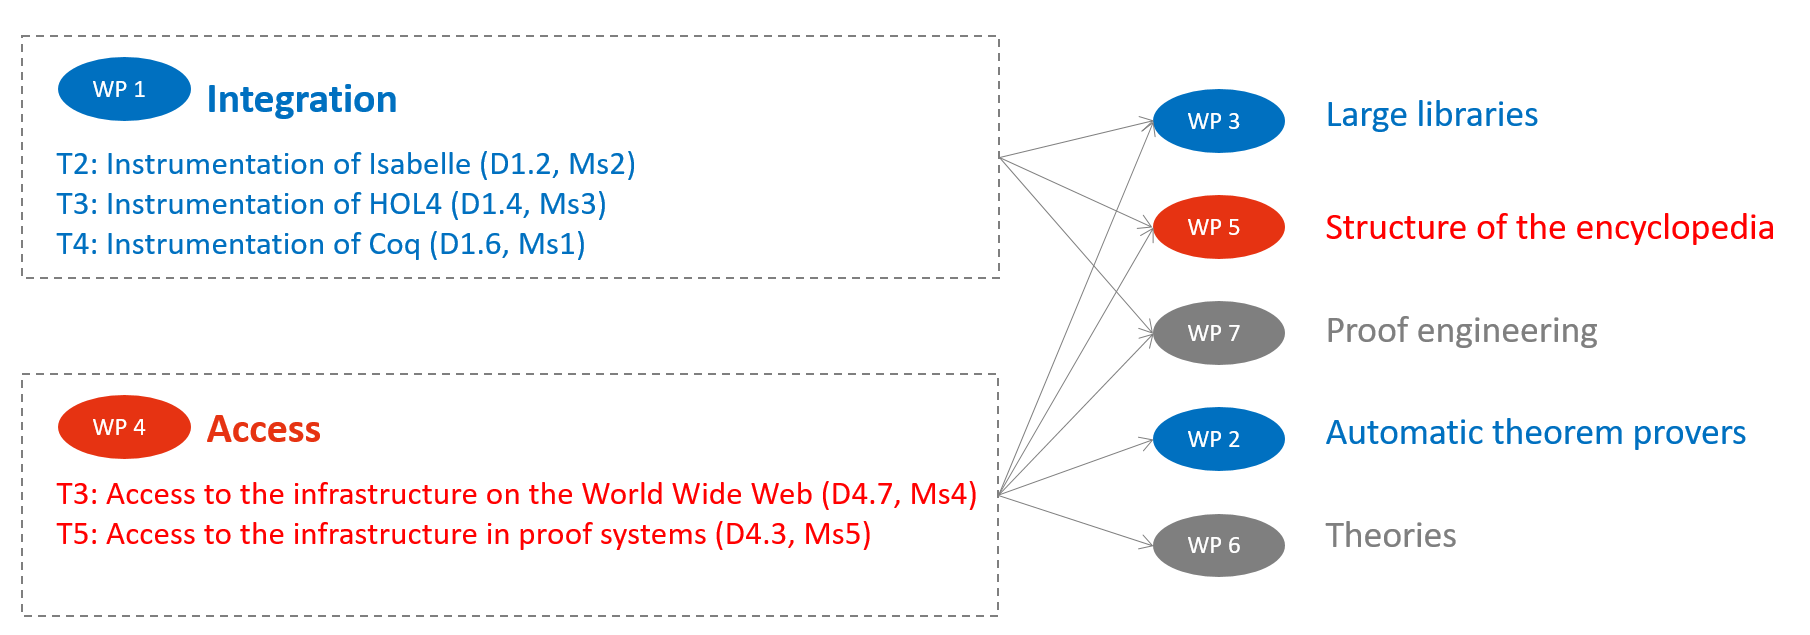
\includegraphics[width=\textwidth]{img/PERT}


%%% Local Variables:
%%%   mode: latex
%%%   mode: flyspell
%%%   ispell-local-dictionary: "english"
%%% End:


\section{Bibliography Concerning the State of the Art, the Research objectives, and the
  Work Programme}\label{sec:bib}

\begin{todo}{from the proposal template}
In this bibliography, list only the works you cite in your presentation of the state of the
art, the research objectives, and the work programme. This bibliography is not the list
of publications. Non-published works must be included with the proposal.
\end{todo}
\printbibliography[heading=empty,notcategory=featured]
% the following will not become part of the public proposal after all most of this is
% technical or confidential.
\ifpublic\else
\section{Requested Modules/Funds}\label{sec:funds}

For each applicant, we apply for funding within the Basic Module.

\subsection{Funding for Staff}\label{sec:positions}

\subsubsection{Research Staff}\label{sec:positions:research}

We apply for the following positions. All run over the entire duration of the proposed project.

\paragraph*{Non-doctoral staff}\ednote{compute amount in elan and copy here}

One doctoral researcher for 2 years at $100 \%$ for Michael Kohlhase.

One doctoral researcher for 2 years at $100 \%$ for Florian Rabe.

%\paragraph*{Postdoctoral staff}
%\ednote{postdoctoral researcher and comparable}

\paragraph*{Other research assistants}\ednote{students with BSc.}

One student with BSc. for 2 years at $100 \%$ for Michael Kohlhase.

One student with BSc. for 2 years at $100 \%$ for Florian Rabe.

\subsubsection{Non-Academic Staff \qquad None.}

\subsubsection{Student Assistants \qquad None.}

\subsection{Funding for Direct Project Costs}\label{sec;funds:direct}

\subsubsection{Equipment up to 10,000 \texteuro, Software and Consumables}

None.  PC will cover the workspace, computing needs, and consumables for its staff as part
of the basic support.

\subsubsection{Travel Expenses}\label{sec:travel}

\begin{oldpart}{rework}
  The travel budget shall cover:
  \begin{itemize}
  \item visits to external collaborators. We expect two international visits. We estimate
    that each visit will be most effective, if the junior researchers can spend about 3
    weeks with the partners. Thus we estimate 2500 {\texteuro} per visit.
  \item visits to national conferences to disseminate the results of {\pn}. We expect
    one visit for each year for each of the three researchers. (3 x 3 x 1000 {\texteuro})
  \item visits to international conferences to disseminate the results of {\pn}. These
    are in particular the International Joint Conference on Document Engineering (DocEng)
    and the Tech User Group Meeting (TUG). We expect one visit for each proposed
    researcher and for each year. (3 x 3 x 1500 {\texteuro})
  \end{itemize}

  This sums up to a total amount of 32.500 {\texteuro} for travel expenses for the whole
  funding period of three years which is split into 16.250 {\texteuro} for each institute
  (PC and Jacobs University).
\end{oldpart}

\subsubsection{Visiting Researchers}\label{sec:funds:visiting}

Total expenses \textbf{10.200 \texteuro}
\medskip

As explained in Section~\ref{sec:travel}, we expect 5 incoming research visits.  Assuming
an average duration of 3 weeks, we estimate the cost of one visit at 600 {\texteuro} for
traveling and 70 {\texteuro} per night for accommodation, amounting to 2040 \texteuro per
visit.

\subsubsection*{-- 4.1.2.6, 4.1.3 (Expenses for Laboratory Animals / Other Costs
/ Project Related Publication Expenses / Instrumentation) \sf\qquad n/a}

% \subsubsection{Expenses for Laboratory Animals} None.
% \subsubsection{Other Costs} None.
% \subsubsection{Project-Related Publication Expenses} None.
% \subsection{Funding for Instrumentation} None.

%%% Local Variables: 
%%% mode: LaTeX
%%% TeX-master: "proposal"
%%% End: 

% LocalWords:  ipower texteuro

\section{Project Requirements}\label{sec:requirements}

\subsection{Employment Status Information}\label{sec:req:employment-status}

\begin{todo}{from the proposal template}
  For each applicant, state the last name, first name, and employment status (including
  duration of contract and funding body, if on a fixed-term contract).
\end{todo}

\subsection{First-time Proposal Data}\label{sec:req:first}

\begin{todo}{from the proposal template}
  Only if applicable: Last name, first name of first-time applicant.

  If this is your first proposal, reviewers will consider this fact when assessing your
  pro- posal. Previous proposals for research fellowships, publication funding, travel
  allow- ances, or funding for scientific networks are not considered first proposals. If
  you are submitting a “first-time proposal” and it is part of a joint proposal, please
  note that your independent project must be distinct from the other projects.

  If you have already submitted a proposal as an applicant for a research grant and have
  received a letter informing you of the funding decision, or if you have led an independ-
  ent junior research group or project in a Collaborative Research Centre or Research
  Unit, you are no longer eligible to submit a “first proposal”. If you have submitted a
  “first-time proposal” and it was rejected, you may resubmit the application, in revised
  form, as a first-time proposal for the same project.
\end{todo}

\subsection{Composition of the Project Group}\label{sec:req:group}

\begin{todo}{from the proposal template}
  List only those individuals who will work on the project but will not be paid out of the
  project funds. State each person’s name, academic title, employment status, and type of
  funding.

  Please list separately the individuals paid by your institution and those paid using
  other third-party funding (including fellowships).
\end{todo}

\begin{sitedescription}{jacu}
  The KWARC (Knowledge Adaptation and Reasoning for Content) research group headed by
  Michael Kohlhase for has the following members
  \begin{compactdesc}
  \item[Dr. N.N.] is the \ldots She has a background in\ldots.
  \end{compactdesc}
  Additionally, the group has attracted about 10 undergraduate and master's students that
  actively take part in the project work and various aspects of research.
\end{sitedescription}

\begin{sitedescription}{pcg}
  Power Consulting GmbH is the leading provider of semantic document solutions. Dr. Senior
  Researcher leads an applied research group consisting of
  \begin{compactdesc}
  \item[Dr. N.N.] is the \ldots She has a background in\ldots.
  \end{compactdesc}
  The group has access to seven programming slaves specializing in web development and
  document transformation techniques
\end{sitedescription}


\subsection{Cooperation with other Researchers}\label{sec:coop}

\subsubsection{Planned Cooperations}\label{sec:coop:planned}
\begin{todo}{from the proposal template}
  Researchers with whom you have agreed to cooperate on this project
\end{todo}
\begin{compactdesc}
\item[Prof. Dr. Super Akquisiteur (Uni Paderborn)] knows exactly what to do to get funding
  with DFG, we will interview him closely and integrate all his intuitions into the {\pn}
  templates.
\item[Prof. Dr. Habe Nichts (Uni Hinterpfuiteufel)] has never gotten a grant proposal
  through with DFG, we will try to avoid his mistakes.
\item[Dr. Sach Bearbeiter (DFG)] will consult with the DFG requirements to be met in the
  proposals.
\item[Dr. Donald Knuth (Stanford University)] is so surprised that we want to do grant
  proposals in {\TeX/\LaTeX} that he will help us with any problems we have in coding in
  this wonderful programming language.
\end{compactdesc}

\subsubsection{Scientific Collaborations in the past Three Years}\label{sec:past-coop}

\begin{todo}{from the proposal template}
  Researchers with whom you have collaborated scientifically within the past three years

  This information will assist the DFG’s Head Office in avoiding potential conflicts of
  in- terest during the review process.
\end{todo}

\subsection{Scientific Equipment}\label{sec:req:equipment}

Jacobs University provides laptops or desktop workstations for all academic
employees. Great Consulting GmbH. is rolling in money anyways and has all of the latest
gadgets.


\subsection{Project-Relevant Interests in Commercial Enterprises\qquad n/a}

%%% Local Variables: 
%%% mode: LaTeX
%%% TeX-master: "proposal"
%%% End: 

% LocalWords:  Durchf uhrung subsubsection ipower Hinterpfuiteufel Sach Aktivit
% LocalWords:  Erkl arungen


\section{Additional Information}\label{sec:additional}

Funding proposal XYZ-83282 has been submitted prior to this proposal on related topic XYZ.
\fi % ifpublic
\end{proposal}
\end{document}
 
%%% Local Variables: 
%%% mode: LaTeX
%%% TeX-PDF-mode:t
%%% TeX-master: t
%%% End: 

% LocalWords:  empty bibflorian systems rabe institutions modal historical pub ednotes
% LocalWords:  kwarc till formalsafe miko gc ipower ipowerlong Antr agen Beitr

% LocalWords:  acrolong intellegible kollaboratives koh arenten ussen Proze pcg
% LocalWords:  Versionsmanagementsystem textsc unterst utzt konzentieren stex
% LocalWords:  mechanik workplan thispagestyle newpage Principcal cvpubsmiko pn
% LocalWords:  ourpubs zusammenfassung printbibliography pubspage ntelligent
% LocalWords:  iting pnlong

% \end{verbatim}
% that amounts to running |proposal.tex| with different options.
% 
% \section{Limitations and Enhancements}\label{sec:limitations}
% 
% The |euproposal| is relatively early in its development, and many enhancements are
% conceivable. We will list them here.
% \begin{enumerate}
% \item none reported yet. 
% \end{enumerate}
% If you have other enhancements to propose or feel you can alleviate some limitation,
% please feel free to contact the author. 
%
% \StopEventually{\newpage\PrintIndex\newpage\PrintChanges\newpage\printbibliography}\newpage
%
% \section{The Implementation}\label{sec:implementation}
%
% In this section we describe the implementation of the functionality of the |euproposal|
% and |eureporting| classes and the |eupdata| package. 
%
% \subsection{Package Options and Format Initialization}\label{sec:impl:options}
% 
% We first set up the options for the package. 
% 
%    \begin{macrocode}
%<*cls>
\newif\ifpartB\partBfalse
\DeclareOption{partB}{\partBtrue}
\newif\if@split\@splitfalse
\DeclareOption{split}{\@splittrue}
\DeclareOption*{\PassOptionsToClass{\CurrentOption}{proposal}}
%</cls>
%<reporting>\DeclareOption*{\PassOptionsToClass{\CurrentOption}{reporting}}
%<cls|reporting>\ProcessOptions
%    \end{macrocode}
%
%    Then we load the packages we make use of
% 
%    \begin{macrocode}
%<cls>\ifpartB\LoadClass[report]{proposal}\else\LoadClass{proposal}\fi
%<reporting>\LoadClass[report]{reporting}
%<*cls|reporting>
\RequirePackage{longtable}
\RequirePackage{eurosym}
\RequirePackage{wrapfig}
\RequirePackage{eupdata}
\RequirePackage{datetime}
%    \end{macrocode}
% we want to change the numbering of figures and tables
%    \begin{macrocode}
\RequirePackage{chngcntr}
\counterwithin{figure}{subsection}
\counterwithin{table}{subsection}
%    \end{macrocode}
%    And finally, we set the section numbering depth, so that paragraphs are numbered and
%    can be cross-referenced.
%    \begin{macrocode}
\setcounter{secnumdepth}{4}
%</cls|reporting>
%    \end{macrocode}
% \subsection{Proposal Metadata and Title Page}\label{sec:impl:metadata}
%  
% We extend the metadata keys from the |proposal| class.
%    \begin{macrocode}
%<*pdata>
\define@key{prop@gen}{coordinator}{\def\prop@gen@coordinator{#1}\pdata@def{prop}{gen}{coordinator}{#1}}
\define@key{prop@gen}{coordinatorsite}{\def\prop@gen@coordinatorsite{#1}\pdata@def{prop}{gen}{coordinator}{#1}}
\def\prop@gen@challenge{??}\def\prop@gen@challengeid{??}
\define@key{prop@gen}{challenge}{\def\prop@gen@challenge{#1}\pdata@def{prop}{gen}{challenge}{#1}}
\define@key{prop@gen}{challengeid}{\def\prop@gen@challengeid{#1}\pdata@def{prop}{gen}{challengeid}{#1}}
\def\prop@gen@objective{??}\def\prop@gen@objectiveid{??}
\define@key{prop@gen}{objective}{\def\prop@gen@objective{#1}\pdata@def{prop}{gen}{objective}{#1}}
\define@key{prop@gen}{objectiveid}{\def\prop@gen@objectiveid{#1}\pdata@def{prop}{gen}{objectiveid}{#1}}
\def\prop@gen@outcome{??}\def\prop@gen@outcomeid{??}
\define@key{prop@gen}{outcome}{\def\prop@gen@outcome{#1}\pdata@def{prop}{gen}{outcome}{#1}}
\define@key{prop@gen}{outcomeid}{\def\prop@gen@outcomeid{#1}\pdata@def{prop}{gen}{outcomeid}{#1}}
\define@key{prop@gen}{callname}{\def\prop@gen@callname{#1}\pdata@def{prop}{gen}{callname}{#1}}
\define@key{prop@gen}{callid}{\def\prop@gen@callid{#1}\pdata@def{prop}{gen}{callid}{#1}}
\define@key{prop@gen}{iconrowheight}{\def\prop@gen@iconrowheight{#1}}
\define@key{prop@gen}{topicsaddressed}{\def\prop@gen@topicsaddressed{#1}}
%</pdata>
%    \end{macrocode}
%
% and now the ones for the final report 
%    \begin{macrocode}
%<*reporting>
\define@key{prop@gen}{reportperiod}{\def\prop@gen@reportperiod{#1}}
\define@key{prop@gen}{key}{\@dmp{key=#1}%
\@ifundefined{prop@gen@keys}{\xdef\prop@gen@keys{#1}}{\xdef\prop@gen@keys{\prop@gen@keys,#1}}}
\define@key{prop@gen}{projpapers}{\def\prop@gen@projpapers{#1}}
%</reporting>
%    \end{macrocode}
% 
% and the default values, these will be used, if the author does not specify something
% better.
%
% If the |propB| option is given, we need to redefine some of the internal counters and
% table of contents mechanisms to adapt to the fact that the proposal text is just Part B.
%
%    \begin{macrocode}
%<*cls>
\ifpartB
\def\thepart{\Alph{part}}
\setcounter{part}{2}
\def\thechapter{\thepart.\arabic{chapter}}
\def\numberline#1{\hb@xt@\@tempdima{#1\hfil} }
\fi
%    \end{macrocode}
% 
% \begin{macro}{\prop@sites@table}
%    \begin{macrocode}
\newcommand\prop@sites@table{\def\@@table{}
{\let\tabularnewline\relax\let\hline\relax
\@for\@I:=\prop@gen@sites\do{\xdef\@@table{\@@table\pdataref{site}\@I{number}}
\xdef\@@table{\@@table&\@nameuse{wa@institution@\@I @name}
\ifx\@I\prop@gen@coordinatorsite (coordinator)\fi}
\xdef\@@table{\@@table&\@nameuse{wa@institution@\@I @acronym}}
\xdef\@@table{\@@table&\@nameuse{wa@institution@\@I @countryshort}\tabularnewline\hline}}}
\begin{tabular}{|l|p{8cm}|l|l|}\hline%|
\# & Participant organisation name & Short name &  Country\\\hline\hline
\@@table
\end{tabular}}
%    \end{macrocode}
% \end{macro}
% 
% \begin{environment}{prop@proposal}
%    \begin{macrocode}
\renewenvironment{prop@proposal}
{\ifgrantagreement\else
  \thispagestyle{empty}\begin{center}
  {\Large \prop@gen@instrument}\\[.2cm]
  {\Large\textbf\prop@gen@callname}\\[.4cm]
  {\LARGE \prop@gen@callid}\\[.8cm]
  {\huge\textbf\prop@gen@title}\\[.4cm]
  \ifx\prop@gen@acronym\@empty\else{\LARGE Acronym: {\prop@gen@acronym}}\\[2cm]\fi
\end{center}
%{\large\prop@gen@instrument}\\
{\large\textbf{Date of Preparation: \today: \currenttime}}
% \ifsubmit\else\if@svninfo\if@gitinfo\\
% {\large\textbf{Revision}: 
% \if@svninfo\svnInfoRevision\fi\if@gitinfo\gitAbbrevHash\fi
%  of 
% \if@svninfo\svnInfoDate\fi\if@gitinfo\gitAuthorDate\fi}
% \fi\fi\fi
\\[1em]
\begin{large}
 \begin{description}
  % \item[Work program topics addressed by \pn:]
  %   \@ifundefined{prop@gen@topicsaddressed}
  %   {\textbf{Challenge \prop@gen@challengeid}: \prop@gen@challenge,
  %   \textbf{Objective \prop@gen@objectiveid}: \prop@gen@objective,
  %   \textbf{target outcome \prop@gen@outcomeid}) \prop@gen@outcome.
  %   {\prop@gen@topicsaddressed}\\[1em]
  \item[Coordinator:] \wa@ref3{person}\prop@gen@coordinator{name}
  \item[e-mail:] \wa@ref3{person}\prop@gen@coordinator{email}
  \item[tel/fax:] \wa@ref3{person}\prop@gen@coordinator{worktelfax}
    \@ifundefined{prop@gen@keywords}{}{\item[Keywords:]  \prop@gen@keywords}
  \end{description}
\end{large}
\vspace*{1em}
\begin{center}
\prop@sites@table\vfill
\@ifundefined{prop@gen@iconrowheight}{}
{\@for\@site:=\prop@gen@sites\do{\wa@institution@logo[height=\prop@gen@iconrowheight]\@site\qquad}}
\end{center}
\newpage
\fi% ifgrantagreement
\setcounter{tocdepth}{2}\setcounter{part}{2}}
{\newpage\printbibliography[heading=warnpubs]%
\if@split
\newwrite\@@SPLIT%
\immediate\openout\@@SPLIT=SPLIT.at%
\protected@write\@@SPLIT{}{\thepage}%
\closeout\@@SPLIT%
\fi}% if@split  
%    \end{macrocode}
% \end{environment}
% 
%    \begin{macrocode}
\def\prop@gen@instrument{Proposal Instrument (e.g. IP)}
%    \end{macrocode}
%
% \subsection{Site Descriptions}\label{sec:sitedesc}
% \ednote {this functionality should probably be refactored into proposal.dtx}
%
% \begin{environment}{sitedescription}
%   \ednote{document this above} |\begin{sitedescritpion}[|\meta{opt}|]{\meta{site}}|
%     marks up the description for the site \meta{site}. It looks up the relevant metadata
%     from the respective |\WAinstitution| declarations.  The options argument \meta{opt}
%     is a key-value list for the keys \DescribeMacro{logo}|logo| (add the logo from
%     |\WAinstitution| to the site description), \DescribeMacro{width}|width|,
%     \DescribeMacro{height}|height| (intended dimensions of the logo), \ednote{more?}.
%    \begin{macrocode}
\define@key{site@desc}{box}[true]{\def\site@desc@box{#1}%
\pdata@def{sitedesc}{\@site}{box}{#1}}
\define@key{site@desc}{logo}[true]{\def\site@desc@logo{#1}%
\pdata@def{sitedesc}{\@site}{logo}{#1}}
\define@key{site@desc}{width}{\def\site@desc@width{#1}%
\pdata@def{sitedesc}{\@site}{width}{#1}\@dmp{wd=#1}}
\define@key{site@desc}{height}{\def\site@desc@height{#1}%
\pdata@def{sitedesc}{\@site}{height}{#1}\@dmp{ht=#1}}
\newenvironment{sitedescription}[2][]%
{\def\c@site{#2}% remember the site ID
\newcounter{site@#2@PM} % for the site PM
\def\site@desc@box{false}% not box unless requested
\def\site@desc@logo{false}% not logo unless requested
\def\site@desc@height{1.3cm}% default height
\def\site@desc@width{5cm}% default width
\setkeys{site@desc}{#1}% read the keys to overwrite the defaults
\ifx\@site@desc@box\@true% if we want a logo
\begin{wrapfigure}{r}{\site@desc@width}\vspace{-2.5ex}%
\begin{tabular}{|p{\site@desc@width}|}\hline\vspace{1mm}%
\ifx\@site@desc@logo\@true% if we want a logo
\wa@institution@logo[height=\site@desc@width]{#2}\\[1ex]%
\fi% end logo
\textbf{\wa@ref3{institution}{#2}{type}.\hfill \wa@ref3{institution}{#2}{country}}\\%
\small\wa@ref3{institution}{#2}{streetaddress}, \wa@ref3{institution}{#2}{townzip}\\\hline%
\end{tabular}\vspace{-2.5ex}%
\end{wrapfigure}%
\fi% end box
\pdata@target{site}{#2}%
{\subsubsection{\wa@ref3{institution}{#2}{acronym}: % space here
{\textsc{\wa@ref3{institution}{#2}{name}}  (\wa@ref3{institution}{#2}{countryshort})}}}%
\small%
\renewcommand\paragraph{\@startsection{paragraph}{4}{\z@}%
                                    {0.25ex \@plus1ex \@minus.2ex}%
                                    {-1em}%
                                    {\normalfont\normalsize\bfseries}}}
{\pdata@def{site}{\c@site}{reqPM}{\csname thesite@\c@site @PM\endcsname}}
%    \end{macrocode}
% \end{environment}
% 
% \begin{environment}{participant}
%   \ednote{document this above} |\begin{picv}[|\meta{PM}|]{\meta{name}}| marks up the CV
%     and metadata about a principal investigator of a site (it can only be use inside a
%     |sitedescription| environment). The first argument \meta{PM} specifies the
%     involvement in person months: a fair estimation this PI will spend on this specific
%     project over its whole duration.
%    \begin{macrocode}
\define@key{site@part}{type}{\def\site@part@type{#1}\@dmp{type=#1}}
\define@key{site@part}{PM}{\def\site@part@PM{#1}\@dmp{PM=#1}}
\define@key{site@part}{salary}{\def\site@part@salary{#1}}%\@dmp{\euro=#1}}
\define@key{site@part}{gender}{\def\site@part@gender{#1}}%\@dmp{\euro=#1}}
\newenvironment{participant}[2][]%
{\def\site@part@type{}\def\site@part@PM{}\def\site@part@salary{}\def\site@part@gender{}%
\setkeys{site@part}{#1}%
\ifx\site@part@PM\@empty\else\addtocounter{site@\c@site @PM}{\site@part@PM}\fi%
\paragraph*{#2\ %
(\ifx\site@part@type\@empty\else\site@part@type\fi%
\ifx\site@part@gender\@empty\else, \site@part@gender\fi%
\ifx\site@part@PM\@empty\else, \site@part@PM~PM\fi%
)}%
\ignorespaces}
{\par\medskip}
%    \end{macrocode}
% \end{environment}
% 
% \subsection{Work Packages, Work Areas, and Deliverables}\label{sec::impl:wpwa}
%
% \begin{environment}{wp*}
%    \begin{macrocode}
\newmdenv[frametitle=Objectives]{wpobjectives}
\newmdenv[frametitle=Description]{wpdescription}
%    \end{macrocode}
% \end{environment}
%
% \begin{environment}{workpackage}
%    
%    \begin{macrocode}
\renewenvironment{workpackage}[1][]
{\begin{work@package}[#1]\medskip\wpheadertable%
\addcontentsline{toc}{subsubsection}{\wp@label\wp@num: \pdataref{wp}\wp@id{title}}}
{\end{work@package}}
%    \end{macrocode}
% \end{environment}
% 
% \begin{macro}{\wpheadertable}
%   We redefine the macro that computes the default work package header table, since there
%   are more sites in a EU proposal, we do this in a tabular form as asked for in the
%   template. We use the internal counter |@sites@po| (sites plus one) for convenience.
%    \begin{macrocode}
\newcounter{@sitespo}\newcounter{@sitespt}
\renewcommand\wpheadertable{%
\wp@sites@efforts@lines%
\setcounter{@sitespo}{\thewp@sites@num}\addtocounter{@sitespo}{1}%
\par\noindent\begin{tabular}{|l|*{\thewp@sites@num}{c|}c|}\hline%
\multicolumn{\the@sitespo}{|l|}{\textbf{\wp@mk@title{\wp@num}: }%
\textsf{\pdata@target{wp}{\wp@id}{\pdataref{wp}\wp@id{title}}}}
&\textbf{Start: }\pdataref{wp}\wp@id{start}\\\hline%
\wp@sites@line\\\hline%
\wp@efforts@line\\\hline%
\end{tabular}\smallskip\par\noindent\ignorespaces}
%    \end{macrocode}
% \end{macro}
%
% \subsection{Milestones and Deliverables}\label{sec:impl:deliverables}
%
% \begin{environment}{wpdelivs}
%   We make the deliverables boxed in EU proposals, this is simple with |mdframed.sty|.
%    \begin{macrocode}
\surroundwithmdframed{wpdelivs}
%    \end{macrocode}
% \end{environment}
%
% \begin{macro}{\milestone}
%    \begin{macrocode}
\define@key{milestone}{verif}{\gdef\mile@verif{#1}\pdata@def{mile}\mile@id{verif}{#1}}
%    \end{macrocode}
% \end{macro}
% 
% \begin{macro}{milestonetable}
% here we do the work, but only if the file |\jobname.deliverables| exists to make sure
% that the deliverables macros are really defined.
%    \begin{macrocode}
\define@key{mst}{caption}{\gdef\mst@caption{#1}}
\define@key{mst}{wname}{\gdef\mst@wname{#1}}
\define@key{mst}{wdeliv}{\gdef\mst@wdeliv{#1}}
\define@key{mst}{wverif}{\gdef\mst@wverif{#1}}
\newcommand\milestonetable[1][]{%
\IfFileExists{./\jobname.deliverables}{% to avoid errors
\message{euproposal.cls: Generating Milestones Table}%
\def\mst@caption{Milestones, Deliverables, and Verification}%
\def\mst@wname{2.5cm}\def\mst@wdeliv{7cm}\def\mst@wverif{4cm}
\setkeys{mst}{#1}%
{\gdef\mst@lines{}%initialize
\let\tabularnewline\relax\let\hline\relax% so they
\let\textbf\relax\let\emph\relax% do not bother us
\edef\@@miles{\pdataref{all}{mile}{ids}}
\@for\@I:=\@@miles\do{
\edef\@delivs{\pdataref@safe{mile}{\@I}{delivs}}%
\def\@@delivs{}
\@for\@J:=\@delivs\do{\xdef\@@delivs{\@@delivs\ \pdataref{deliv}\@J{label}}}
\def\@@line{
\textbf{\pdataref{mile}\@I{label}}&
\emph{\pdataref{mile}{\@I}{title}} &
\@@delivs&
\pdataref{mile}\@I{month} &
\pdataref{mile}\@I{verif}}
\xdef\mst@lines{\mst@lines\@@line\tabularnewline\hline}}}
\begin{table}[ht]
\begin{tabular}{|l|p{\mst@wname}|p{\mst@wdeliv}|l|p{\mst@wverif}|}\hline
\#&\textbf{\miles@legend@name}
&\textbf{\miles@legend@involved}
&\textbf{\miles@legend@mo}
&\textbf{\miles@legend@verif}\\\hline\hline
\mst@lines
\end{tabular}
\caption{\mst@caption\ ($^\ast$\miles@legend)}\label{tab:milestonetable}
\end{table}}
{\ClassWarning{not formatting mile stones table yet, deliverables are
  still missing; generate\jobname.deliverables\ to get it!}}}
%    \end{macrocode}
% now the multilinguality support 
%    \begin{macrocode}
\newcommand\miles@legend@name{Name}
\newcommand\miles@legend@mo{Mo}
\newcommand\miles@legend@verif{Means of Verif.}
\newcommand\miles@legend@involved{WPs$^\ast$/Deliverables involved}
\newcommand\miles@legend{WP is first number in deliverable label}
%    \end{macrocode}
% \end{macro}
%
% \begin{macro}{\prop@milesfor}
%    the due date is the first argument to facilitate sorting
%    \begin{macrocode}
\newcommand\prop@milesfor[1]{\edef\@delivs{\pdataref@safe{mile}{#1}{delivs}}%
\let\m@sep=\relax\def\new@sep{,\ }%
\@for\@I:=\@delivs\do{\m@sep\pdataRef{deliv}\@I{label}\let\m@sep=\new@sep}}
%    \end{macrocode}
% \end{macro}
% 
% \subsection{Risks}\label{sec:impl:risks}
% 
% \begin{environment}{risk}
%    \begin{macrocode}
\newenvironment{risk}[3]
{\paragraph{Risk: #1}\hfill\emph{probability}: #2, \emph{gravity}: #3\par\noindent\ignorespaces}
{}
%    \end{macrocode}
% \end{environment}
%
% \begin{environment}{riskcont}
%    \begin{macrocode}
\newenvironment{riskcont}[3]
{\begin{risk}{#1}{#2}{#3}\textbf{Contingency:} }
{\end{risk}}
%    \end{macrocode}
% \end{environment}
%
% \subsection{Relevant Papers}\label{sec:impl:papers}
% 
% \begin{macro}{\keypubs}
% we just use the {bib\LaTeX} |refsection| facility. NOTE, this needs biber to work
% easily.
%    \begin{macrocode}
\newcommand\keypubs[1]{%
\begin{refsection}\nocite{#1}\printbibliography[heading=empty]\end{refsection}}
%</cls>
%    \end{macrocode}
% \end{macro}
%
% \Finale
\endinput
% LocalWords:  iffalse cls euproposal euproposal.dtx tt maketitle newpage wpwa eudata dfg
% LocalWords:  tableofcontents ednote euproposal DescribeEnv compactitem impl eureporting
% LocalWords:  longtable eurosym pdata thepart setcounter env vfill qquad NeedsTeXFormat
% LocalWords:  thechapter newcommand tabularnewline hline xdef pdataref nameuse SciML gen
% LocalWords:  countryshort rpoposal clange wrapfig wrapfigure vspace bfseries eupdata wd
% LocalWords:  startsection normalfont normalsize baselinestretch callname hb newpart wp
% LocalWords:  countryshort rpoposal clange wrapfig renewenvironment worktelfax prop@gen
% LocalWords:  tocdepth wpobjectives newenvironment noindent boxedminipage fbox warnpubs
% LocalWords:  textwidth textbf wpdescription sitedescription pgfdeclareimage projpapers
% LocalWords:  wrapfigure vspace pgfuseimage streetaddress townzip textsc xt wa maxnames
% LocalWords:  renewcommand startsection normalfont normalsize bfseries wptitle sitedesc
% LocalWords:  workpackage subsubsection wpheadertable newcounter sitespo hfil if@svninfo
% LocalWords:  newcounter sitespt addtocounter textsf smallskip ignorespaces pn setkeys
% LocalWords:  cellcolor lightgray keypubs paperlist callname callid callid ifx csname
% LocalWords:  challengeid challengeid objectiveid objectiveid outcomeid hfill if@gitinfo
% LocalWords:  outcomeid metakeys workaddress numberline tempdima ifsubmit iconrowheight
% LocalWords:  proposal.dtx texttt paperslist workaddress.dtx topicsaddressed thesite mst
%  LocalWords:  topicsaddressed iconrowheight finalreport.tex printbibliography endcsname
%  LocalWords:  reportperiod organisation thispagestyle gitAbbrevHash sitedescritpion WPs
%  LocalWords:  WAinstitution picv medskip newmdenv frametitle wpdelivs mdframed.sty emph
%  LocalWords:  surroundwithmdframed emph riskcont prob grav ldots endinput optimized

% Local Variables:
% mode: doctex
% TeX-master: t
% End:
%  LocalWords:  coordinatorsite coordinatorsite verif verif milestonetable milestonetable
%  LocalWords:  wname wname wdeliv wdeliv wverif wverif biblatex notcategory newif gdef
%  LocalWords:  grantagreement Initialization ifpartB partBfalse partBtrue report openout
%  LocalWords:  chngcntr counterwithin ifgrantagreement currenttime mst@caption delivs
%  LocalWords:  initialize deliv multilinguality prop@milesfor refsection nocite doctex
%  LocalWords:  secnumdepth newwrite thepage jobname.deliverables
